
\chapter{Multi-core Communication}
\startcontents[chapters]
\printcontents[chapters]{}{1}{}

\noindent\\
So far we have discussed the features and design of the Vmicro16 system-on-chip. This section will discuss the multi-processing functionality of the design and how to use it.

\section{Introduction}
\subsection{Design Goals}
\section{Multi-Processing}
\subsection{Overview}


\begin{figure}[h]
\centering
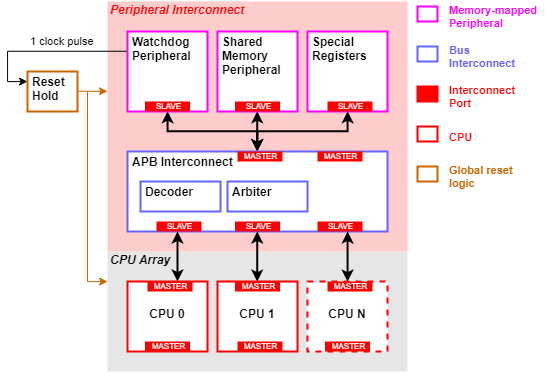
\includegraphics[width=0.7\textwidth]{multicore}
\caption{Block digram showing the main multi-processing components: the CPU array and a peripheral interconnect used for core synchronisation.}
\label{}
\end{figure}

\subsection{Thread Synchronisation}
\subsection{Context Identification}

\section{Design Challenges}
\subsection{Memory Constraints}


\begin{figure}[H]
\centering
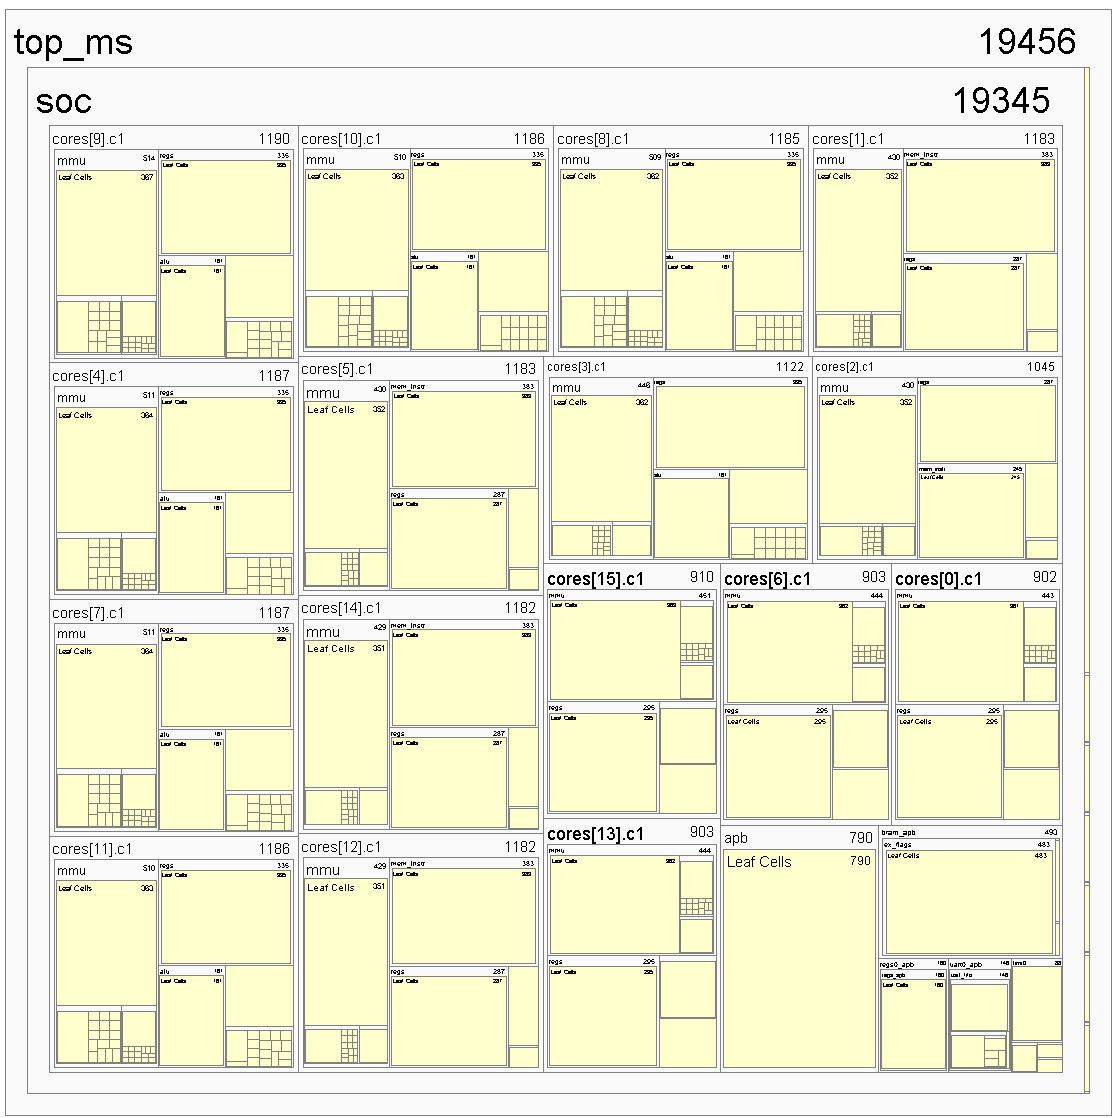
\includegraphics[width=13cm]{soc_layout_schem}
\caption{•}
\label{}
\end{figure}